\documentclass[14pt]{extarticle}

\usepackage[LGR]{fontenc}
\usepackage[main=greek,english]{babel}
\usepackage[utf8]{inputenc}
\usepackage[unicode]{hyperref}
\usepackage{titlepic}
\usepackage{graphicx}
\usepackage{listings}
\usepackage{xcolor}
\usepackage{amsmath}

\graphicspath{ {./img/} }


\hyphenpenalty=10000
\hbadness=10000

\definecolor{codegreen}{rgb}{0,0.6,0}
\definecolor{codegray}{rgb}{0.5,0.5,0.5}
\definecolor{codepurple}{rgb}{0.58,0,0.82}
\definecolor{backcolour}{rgb}{0.95,0.95,0.92}

\lstdefinestyle{mystyle}{
    backgroundcolor=\color{backcolour},   
    commentstyle=\color{codegreen},
    keywordstyle=\color{magenta},
    numberstyle=\tiny\color{codegray},
    stringstyle=\color{codepurple},
    basicstyle=\ttfamily\footnotesize,
    breakatwhitespace=false,         
    breaklines=true,                 
    captionpos=b,                    
    keepspaces=true,                 
    numbers=left,                    
    numbersep=5pt,                  
    showspaces=false,                
    showstringspaces=false,
    showtabs=false,                  
    tabsize=2
}

\lstset{frame=shadowbox, framexleftmargin=4mm, rulesepcolor=\color{black}, style=mystyle}

\title{\bf Εργασία Μεταγλωττιστών \\ Τμήμα Α2}
\titlepic{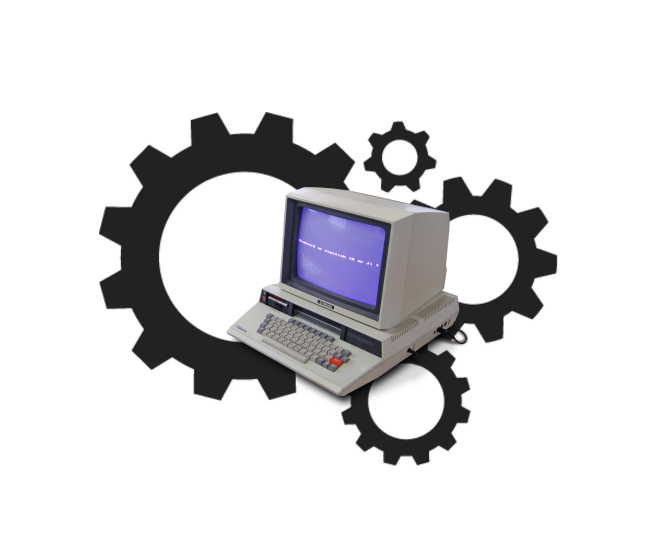
\includegraphics[scale=2.5]{computer.png}}
\author{
  \emph{Ομάδα 15}
}

\begin{document}

\begin{titlepage}
  \maketitle
  \begin{center}
    \large \emph{Ομάδα 15}
    \\
    Αναλυτικά τα μέλη:
\vspace{5mm}
  \begin{tabular}{r l}
    \\Διονύσης Νικολόπουλος & $AM: 18390126$
    \\Θανάσης Αναγνωστόπουλος & $AM: 18390043$
    \\Αριστείδης Αναγνωστόπουλος & $AM: 16124$
    \\Σπυρίδων Φλώρος & $AM: 141084$
  \end{tabular}
\vspace{5mm}
    \\
    Αναλυτικά οι ρόλοι:
    \\
\vspace{5mm}
  \begin{tabular}{r l}
    \small Γενικός Συντονιστής:   Διονύσης Νικολόπουλος
    \\
    \small Υπεύθυνος Τμήματος Εργασίας Α2: Διονύσης Νικολόπουλος
  \end{tabular}
\vspace{5mm}
\\
  \textlatin{Usernames} στο \textlatin{Github}
\\
  \vspace{5mm}
  \begin{tabular}{r l}
    \small Διονύσης Νικολόπουλος : \textlatin{jiud}
    \\
    \small Θανάσης Αναγνωστόπουλος : \textlatin{ThanasisAnagno}
    \\
    \small Αριστείδης Αναγνωστόπουλος : \textlatin{Aris-Anag}
    \\
    \small Σπυρίδων Φλώρος : \textlatin{spirosfl}
  \end{tabular}
  \\
\vspace*{\fill}
    \footnotesize{Η εργασία αυτή πραγματοποιήθηκε με χρήση \LaTeX}
  \end{center}
\end{titlepage}

\tableofcontents
\clearpage

\section{Εισαγωγή}
\large{\bfΤι πραγματεύεται η εργασία}
\\
Στην εργαστηριακή εργασία αυτή ασχοληθήκαμε με την δημιουργία ενός ντετερμινιστικού αυτόματου πεπερασμένων καταστάσεων.
\\
\\
\large{\bfΟ σκοπός του αυτομάτου}
\\
Το αυτόματο αυτό έχει ως σκοπό να λειτουργεί σαν Λεκτικός Αναλυτής της γλώσσας \textlatin{Uni-C}, ενός παρακλαδιού της γλώσσας \textlatin{C}, απο το Πανεπιστήμιο Δυτικής Αττικής.  
\\
\\
\large{\bfΒήματα Υλοποίησης}
\\
Πριν πραγματοποιηθεί φυσικά η κωδικοποίηση για την προσσέγγιση του προβλήματος αυτόυ, έγινε η περιγραφή της γλώσσας \textlatin{Uni-C} σε μορφή \textlatin{BNF}. 
\\
\\
Η κωδικοποίηση του έχει γίνει καταρχήν με την βοήθεια του προγράμματος \emph{\textlatin{FSM}}, που επίσης είναι προγραμματισμένο πάνω στην γλώσσα \textlatin{C}.
\\
\\
Ο σχεδιασμός των διαγραμμάτων έχει γίνει με το πρόγραμμα \emph{\textlatin {JFLAP}}.
\\
\\
\\
\\
\large{\bfΣελίδα στο \textlatin{Github}}
\\
\\
Η σελίδα μας στο \textlatin{Github}, με την οποία διοργανώσαμε την εργασία και δουλέψαμε όλοι μαζί είναι (κάντε κλικ για το λινκ):
\begin{center}
  \textlatin{
  \href{https://github.com/jiud/uni-C-Analyser}{Uni-C-Analyser}
}
\end{center}
Μπορείτε να δείτε αναλυτικά όλη μας την πρόοδο εκεί.
  \\
  \\
\large{\bfΕξήγηση για το τι ακολουθεί}
\\
Σε αυτό το \textlatin{PDF} αρχικά θα παρατεθεί η περιγραφή της \textlatin{Uni-C} σε \textlatin{BNF}.
\\
\\
Έπειτα, θα παρατεθούν επίσης και τα διαγράμματα του εναίου αυτόματου που βοηθούν στην κωδικοποίηση του αλλά και στην σύλληψη νοητά του τι περιμένουμε να κάνει το αυτόματό μας, πως θα το υλοποιήσουμε τεχνικά. 
\\
\\
Στην συνέχεια, θα ακολουθήσει ο κώδικας του αυτόματου τμηματικά με εξηγήσεις της λειτουργίας του.
\\
\\
Τελος, εφόσον ο κώδικας παραδωθεί και ολοκληρωμένα, θα παρατεθούν ορισμένοι ελέγχοι πραγματικής λειτουργίας του αυτόματου σε εικόνες, καταλίγοντας και σε εικόνες που αποδεικνουν ότι οι έλεγχοι έγιναν.


\clearpage
\section{Περιγραφή σύνταξης της \textlatin{Uni-C} σε \textlatin{BNF}}
Πριν την υλοποίηση του αυτομάτου σε εκτελέσιμο κώδικα, όπως αναφέραμε παραπάνω, έγινε η ανάλυση της σύνταξης της γλώσσας \textlatin{Uni-C} σε μορφή \textlatin{BNF (Backus-Naur Form} ή Μορφή Μπάκους-Ναούρ).
\\
Οπότε, με την βοήθεια του περιβάλλοντος λεκτικού επεξεργαστή \textlatin{Emacs}, γράψαμε τον εξής συμβολισμό.   

\selectlanguage{english}
    \begin{lstlisting}[bnf]
symbol        ::= "|" | " " | "!" | "#" | "$" | "%" | "&" | "(" | ")" | "*" | "+" | "," | "-" | "." | "/" | ":" | "\;" | ">" | "=" | "<" | "?" | "@" | "[" | "\" | "]" | "^" | "_" | "`" | "{" | "}" | "~"
letter        ::= "A" | "B" | "C" | "D" | "E" | "F" | "G" | "H" | "I" | "J" | "K" | "L" | "M" | "N" | "O" | "P" | "Q" | "R" | "S" | "T" | "U" | "V" | "W" | "X" | "Y" | "Z" | "a" | "b" | "c" | "d" | "e" | "f" | "g" | "h" | "i" | "j" | "k" | "l" | "m" | "n" | "o" | "p" | "q" | "r" | "s" | "t" | "u" | "v" | "w" | "x" | "y" | "z"
digit         ::= "0" | "1" | "2" | "3" | "4" | "5" | "6" | "7" | "8" | "9"
character     ::= letter | symbol | digit
character1    ::= character | "'"
character2    ::= character | '"'
text1         ::= "" | character1 text1
text2         ::= '' | character2 text2
literal       ::= '"' text1 '"' | "'" text2 "'"
identifier    ::= character text1
operator      ::= "+" | "-" | "*" | "/" | "%" | "=" | "+=" | "-=" | "*=" | "" | "" | "--" | "=" | "=" | "&" | "==" | "!=" | "++" | "&&" | "||"
number1       ::= digit number1 | "'"
number2       ::= digit number2 | '"'
number        ::= number1 | number2
integer       ::= number | "0X" number | "0x" number | "0"  
float         ::= number "." number | number "e" number | number "e" number "-" number
    \end{lstlisting}
\selectlanguage{greek}



\clearpage
\section{Διαγράμματα Ενιαίου Αυτόματου}
\subsection{Γενικευμένο Διάγραμμα Ενιαίου Αυτόματου}
\smallΕδώ είναι το γενικευμένο ενιαίο αυτόματο που σχεδιάσαμε:
\begin{figure}[h!]
  \caption{Γενικευμένο Αυτόματο}
  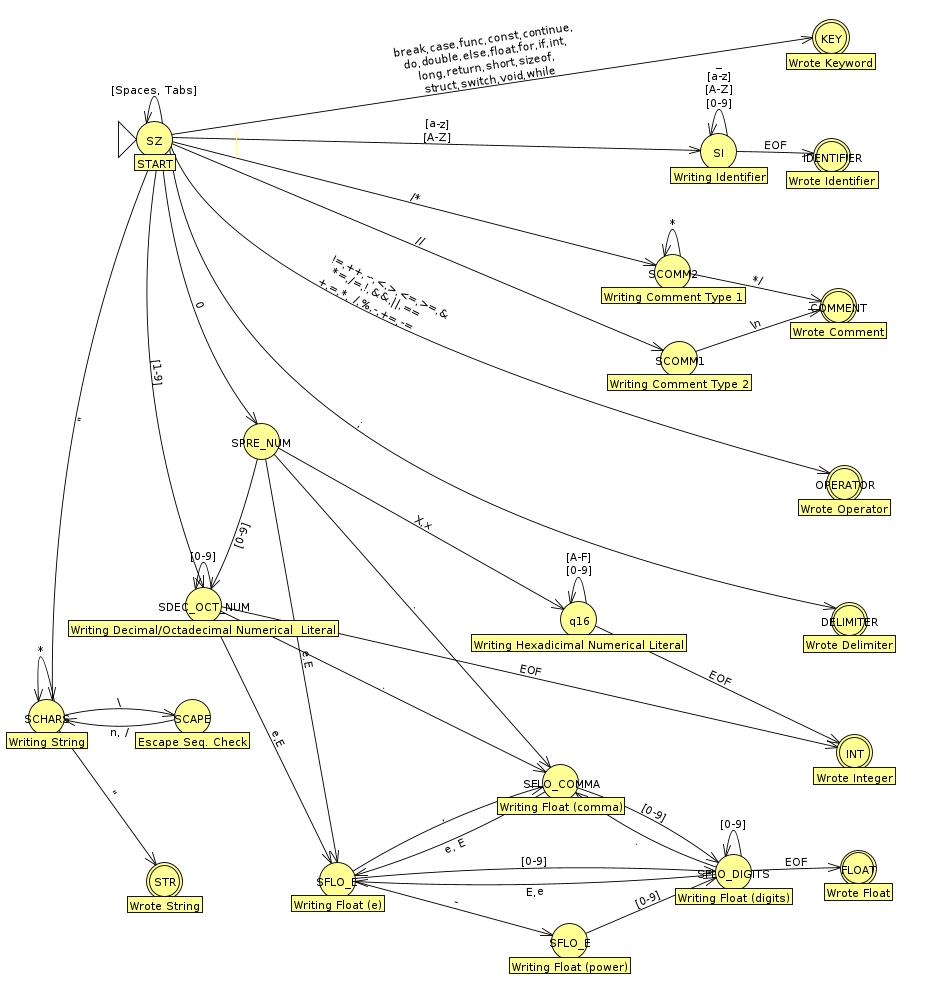
\includegraphics[width=0.9\textwidth]{automata_general}
\end{figure}
\clearpage
\subsection{Λεπτομερές Διάγραμμα Ενιαίου Αυτόματου}
\smallΕδώ είναι το λεπτομερές ενιαίο αυτόματο που σχεδιάσαμε:
\begin{figure}[h!]
  \caption{Λεπτομερές Αυτόματο}
  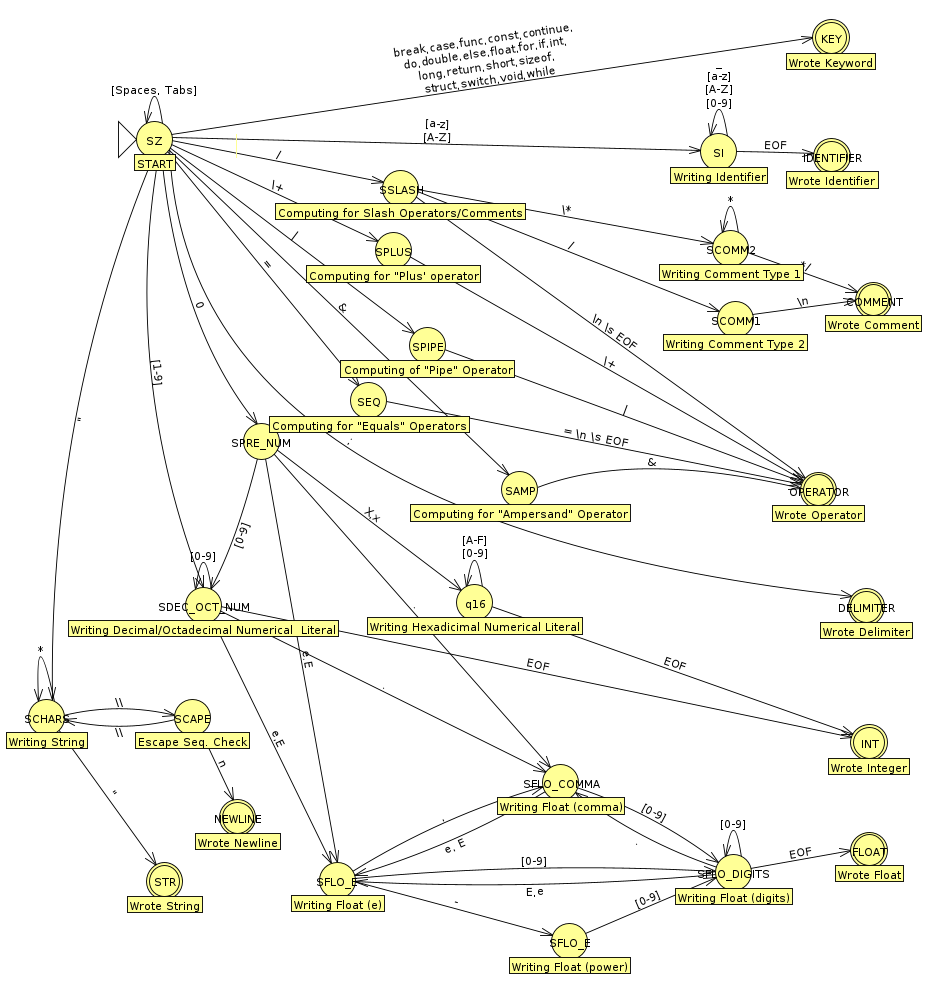
\includegraphics[width=1\textwidth]{automata_detailed}
\end{figure}

\clearpage
\section{Εξήγηση Κώδικα σε \textlatin{FSM}}
Το πρώτο κομμάτι κώδικα σε \textlatin{FSM} είναι, ασφαλώς, η αρχική μας κατάσταση:
\selectlanguage{english}
    \begin{lstlisting}
START=SZ
SZ: % -> OPERATOR
    ! < > \- = \* -> SEQ
    \+ -> SPLUS
    & -> SAMP
    ; -> DELIMITER
    | -> SPIPE
    a-z A-Z _ -> SI
    \n \s -> SZ
    / -> SSLASH
    " -> SCHARS
    0 -> SPRE_NUM
    1-9 -> SDEC_OCT_NUM
    * -> BAD
    EOF -> GOOD
    \end{lstlisting}
\selectlanguage{greek}
Εδώ, βλέπουμε ότι ο αναλυτής μας περιμένει τον πρώτο, ουσιαστικά χαρακτήρα απο τον χρήστη, ο οποίος θα έχει μεγάλη σημασία στο να καθορίσουμε "τι πάει να γράψει ο χρήστης".
\\
\\
Βλέπουμε πολλές καταστάσεις, των οποίων η φιλοσοφία εξηγείται ως εξής.
\begin{itemize}
  \item Οι καταστάσεις που το όνομα τους αρχίζει με \textlatin{"S"} είναι για τον αναλυτή μας οι "μεταβατικές" μας καταστάσεις, οι καταστάσεις στις οποίες δεν έιναι απόλυτα σίγουρο το τι θέλει να γράψει ο χρήστης, αλλά είναι σίγουροι, με βάση κανόνες και ντετερμινιστικά οι "δρόμοι" που μπορεί να ακολουθήσει ο χρήστης. 
  \item Οι υπόλοιπες καταστάσεις, καταστάσεις όπως η \textlatin{DELIMITER} που βλέπουμε εδώ, εκφράζουν επιστροφή του αναγνωριστικού (και άρα επιτυχής αναγνώριση) της λεκτικής μονάδας (πχ εδώ το \textlatin{token} (λεκτική μονάδα) είναι \textlatin{DELIMETER}) καθώς ο αναλυτής μας είναι σίγουρος, \emph{με βάση κανόνες που ακολουθεί ντετερμινιστικά}, ότι η λέξη η οποία ο χρήστης εισήγαγε είναι ενός συγκεκριμένου τύπου.  
\end{itemize}
\clearpage
Συνεχίζοντας, βλέπουμε 2 καταστάσεις που αφορούν την αναγνώριση συμβολοσειράς, στις οποίες είναι δυνατόν να μεταβεί το αυτόματο, αν ο χρήστης εισάγει σε ορισμένες καταστάσεις τον χαρακτήρα \boxed{ "}.
\\
\\
Αυτό ισχύει για την αρχική κατάσταση, όπως είδαμε παραπάνω, αλλά και για τις καταστάσεις \textlatin{IDENTIFIER, INT, FLOAT}, αφού είναι πιθανό ο χρήστης να γράφει μια συμβολοσειρά έπειτα απο τους τύπους λέξεων αυτούς.
\\
\\
Η κατάσταση \textlatin{SCHARS} συγκεκριμένα είναι αυτή στην οποία δίνονται οι χαρακτήρες της συμβολοσειράς, και αφήνεται ένα ενδεχόμενο είτε να τερματισθεί η συμβολοσειρά με το να εισαχθεί ξανά ο χαρακτήρας \boxed{"} (και να μεταβεί στην κατάσταση \textlatin{STR}), είτε να να εισαχθεί ο χαρακτήρας \textbackslash.
\\
\\
Στην τελευταία περίπτωση, ο αναλυτής έρχεται στην κατάσταση \textlatin{SCAPE}, την οποία περιμένει να εισαχθέι είτε ο χαρακτήρας \boxed{\textlatin{n}}, οπότε να επιστραφεί η κατάσταση \textlatin{NEWLINE}, είτε να εισαχθεί ο χαρακτήρας \textbackslash  ξανά, οπότε να επιστρέψει στην κατάσταση \textlatin{SCHARS}, είτε να κάνει λάθος και να εισαχθεί οποιοσδήποτε άλλος χαρακτήρας, οπότε να παέι στην κατάσταση \textlatin{BAD}.  
\\
\\
Στην κατάσταση \textlatin{NEWLINE}, οποιοσδήποτε χαρακτήρας μας πάει πίσω στην κατάσταση \textlatin{SCHARS}, ενώ ο χαρακτήρας \boxed{"} στην κατάσταση \textlatin{STR}
\\
\selectlanguage{english}
    \begin{lstlisting}
SCHARS: * -> SCHARS
        " -> STR
        \\ -> SCAPE

SCAPE:  n -> NEWLINE
        \\ -> SCHARS
        * -> BAD

NEWLINE: " -> STR
         * -> SCHARS 

STR:        \s \n -> SZ
            ;     -> DELIMITER
            EOF   -> GOOD
    \end{lstlisting}
\selectlanguage{greek}

\clearpage
Με παρόμοια λογική βλέπουμε διάφορους χαρακτήρες που είναι \emph{δυνητικά} τελεστές (ο πρώτος είναι δυνητικά και σχόλιο).
\selectlanguage{english}
    \begin{lstlisting}
SSLASH: / -> SCOMM1
        = \n \s -> OPERATOR
        \* -> SCOMM2
         * -> BAD
    
SEQ:     = \n \s -> OPERATOR
         * -> BAD

SPLUS:   = \+  -> OPERATOR
         * -> BAD

SAMP:    & \s  -> OPERATOR
         * -> BAD

SPIPE:   |     -> OPERATOR
         * -> BAD
    \end{lstlisting}
\selectlanguage{greek}
\\   
Επίσης, εδώ βλέπουμε, με παρόμοιο συλλογισμό με τις καταστάσεις για τις συμβολοσειρές, και την επεξεργασία για τα σχόλια (με τελική κατάσταση την κατάσταση \textlatin{COMMENT})
\selectlanguage{english}
    \begin{lstlisting}
SCOMM1:     * -> SCOMM1
           \n -> SZ

SCOMM2:    \* -> SCOMM21
           * -> SCOMM2
            
SCOMM21:    / -> COMMENT
            * -> SCOMM2

COMMENT:    \n \s -> SZ  
            EOF -> GOOD
    \end{lstlisting}
\selectlanguage{greek}
\\
Παρατηρούμε και την κατάσταση \textlatin{SI}, η οποία δέχεται τους επιτρεπτούς χαρακτήρες ως κομμάτια της πιθανής λέξης ενός \textlatin{identifier}, που με τον χαρακτηρα \boxed{;}, με κενό, ή με τέλος αρχείου γίνεται η μεταβολή του αναλυτή στην κατάσταση \textlatin{IDENTIFIER}.
\selectlanguage{english}
    \begin{lstlisting}
SI:      a-z A-Z 0-9 _ -> SI
         ;             -> IDENTIFIER
         \s            -> IDENTIFIER 
         EOF           -> IDENTIFIER
         \+ \- =       -> IDENTIFIER
         * -> BAD
    \end{lstlisting}
\selectlanguage{greek}

Εδώ βλέπουμε τις "τελικές" καταστάσεις στις οποίες φτάνει ο αναλυτής οταν κρίνει μια λέξη να πληρεί τις προϋποθέσεις για να χαρακτηρισθεί ως μια συγκεκριμένη λεκτική μονάδα.
\\
Παρατηρούμε ότι, με βάση την γλώσσα \textlatin{Uni-C}, οι λεκτικές μονάδες είναι δυνατό να ακολουθηθούν απο συγκεκριμένες λεκτικές μονάδες (παράδειγμα οι τελεστές μονάχα από ένα νούμερο ή \textlatin{identifier}, για αυτό οι μοναδικές επιτρεπτές καταστάσεις που μεταβαίνει ο αναλυτής μετά απο την κατάσταση \textlatin{OPERATOR} είναι η ενδιάμεση κατάσταση έιτε αριθμού έιτε \textlatin{identifier}) 
\selectlanguage{english}
    \begin{lstlisting}
 OPERATOR:  a-z A-Z _ -> SI
            0 -> SPRE_NUM
            1-9 -> SDEC_OCT_NUM    
            " -> SCHARS
            * -> BAD
            \s -> SZ

DELIMITER:  * -> SZ
INT:        \s \n -> SZ
            A-Z a-z _ -> SI
            % -> OPERATOR
            ! < > \- = \* -> SEQ
            \+ -> SPLUS
            & -> SAMP
            ; -> DELIMITER
            | -> SPIPE
            / -> SSLASH
            0 -> SPRE_NUM
            1-9 -> SDEC_OCT_NUM
            * -> BAD
            " -> SCHARS
            EOF -> GOOD

FLOAT:      \s \n -> SZ
            A-Z a-z _ -> SI
            % -> OPERATOR
            ! < > \- = \* -> SEQ
            \+ -> SPLUS
            & -> SAMP
            ; -> DELIMITER
            | -> SPIPE
            / -> SSLASH
            0 -> SPRE_NUM
            1-9 -> SDEC_OCT_NUM
            * -> BAD
            EOF -> GOOD
    
IDENTIFIER: \s \n -> SZ
            A-Z a-z _ -> SI
            % -> OPERATOR
            ! < > \- = \* -> SEQ
            \+ -> SPLUS
            & -> SAMP
            ; -> DELIMITER
            | -> SPIPE
            / -> SSLASH
            0 -> SPRE_NUM
            1-9 -> SDEC_OCT_NUM
            * -> BAD
            " -> SCHARS
            EOF -> GOOD


    \end{lstlisting}
\selectlanguage{greek}

\clearpage
Τέλος, έχουμε τις ενδιάμεσες καταστάσεις με τις οποίες ο αναλυτής κρίνει αν ο αριθμός που εισάγεται είναι πραγματικός ή ακέραιος.
\\
Με βάση λοιπόν την σύνταξη της \textlatin{Uni-C}, διαχωρίζονται αυτές οι δυό κατηγορίες.
\\
(πχ. ακέραιοι: 0, 954, 4235 πχ. πραγματικοί: 3.14 2.43Ε31, 35.3\textlatin{e}10, 34\textlatin{e}12, 0\textlatin{e}0, 0.2222)  
\selectlanguage{english}
    \begin{lstlisting}
SPRE_NUM:   x X -> SHEX
            0-9 -> SDEC_OCT_NUM
            \.  ->  SFLO1
            e E -> SFLO2
            *   -> BAD
            \s  -> INT
            
SDEC_OCT_NUM:   0-9     -> SDEC_OCT_NUM
                \.      -> SFLO_COMMA
                e E     -> SFLO_E
                \s \n ; -> FLOAT
                * -> BAD

SFLO_COMMA:     \s \n ; -> FLOAT
                e E     -> SFLO_E
                0-9     -> SFLO_DIGITS
                * -> BAD

SFLO_DIGITS:    0-9     -> SFLO_DIGITS
                \n \s ; -> FLOAT
                e E     -> SFLO_E
                \.      -> SFLO_COMMA
                * -> BAD

SFLO_E:         \.       -> SFLO_COMMA
                \-       -> SFLO_POWER 
                0-9     -> SFLO_DIGITS
                * -> BAD

SFLO_POWER:     0-9     -> SFLO_DIGITS
                * -> BAD
    
SHEX:       A-F     -> SHEX
            0-9     -> SHEX
            \s \n ; -> INT
            * -> BAD
    \end{lstlisting}
\selectlanguage{greek}


\clearpage
\section{Ολοκληρωμένος Κώδικας σε \textlatin{FSM}}
Ο κώδικας του αυτοματού μας μπορεί να βρεθεί ως αρχείο και στον φάκελο \textlatin{\boxed{Source\_Code}} που βρήκεται μέσα στον κύριο φάκελο του παραδοτέου.
\\
\small Ακολουθεί ο ολοκληρωμένος κώδικας σε \textlatin{FSM} του αυτόματού μας:  
\selectlanguage{english}
    \begin{lstlisting}
START=SZ
SZ: % -> OPERATOR
    ! < > \- = \* -> SEQ
    \+ -> SPLUS
    & -> SAMP
    ; -> DELIMITER
    | -> SPIPE
    a-z A-Z _ -> SI
    \n \s -> SZ
    / -> SSLASH
    " -> SCHARS
    0 -> SPRE_NUM
    1-9 -> SDEC_OCT_NUM
    * -> BAD
    EOF -> GOOD


SCHARS: * -> SCHARS
        " -> STR
        \\ -> SCAPE

SCAPE:  n -> NEWLINE
        \\ -> SCHARS
        * -> BAD

NEWLINE: " -> STR
         * -> SCHARS 
    
SSLASH: / -> SCOMM1
        = \n \s -> OPERATOR
        \* -> SCOMM2
    
SEQ:     = \n \s -> OPERATOR
        * -> BAD

SPLUS:   = \+  -> OPERATOR
        * -> BAD

SAMP:    & \s  -> OPERATOR
        * -> BAD

SPIPE:   |     -> OPERATOR
        * -> BAD

SI:      a-z A-Z 0-9 _ -> SI
         ;           -> IDENTIFIER
         \s \n       -> IDENTIFIER 
         EOF         -> IDENTIFIER
         \+ \- =     -> IDENTIFIER
         * -> BAD
        
SCOMM1:     * -> SCOMM1
           \n -> SZ

SCOMM2:    \* -> SCOMM21
           * -> SCOMM2
            
SCOMM21:    / -> COMMENT
            * -> SCOMM2

COMMENT:    \n \s -> SZ  

OPERATOR:   a-z A-Z _ -> SI
            0 -> SPRE_NUM
            1-9 -> SDEC_OCT_NUM    
            " -> SCHARS
            * -> BAD
            \s -> SZ

DELIMITER:  * -> SZ

SPRE_NUM:   x X -> SHEX
            0-9 -> SDEC_OCT_NUM
            \.  ->  SFLO1
            e E -> SFLO2
            *   -> BAD
            \s  -> INT
            
SDEC_OCT_NUM:   0-9     -> SDEC_OCT_NUM
                \.      -> SFLO_COMMA
                e E     -> SFLO_E
                \s \n ; -> FLOAT
                * -> BAD

SFLO_COMMA:     \s \n ; -> FLOAT
                e E     -> SFLO_E
                0-9     -> SFLO_DIGITS
                * -> BAD

SFLO_DIGITS:    0-9     -> SFLO_DIGITS
                \n \s ; -> FLOAT
                e E     -> SFLO_E
                \.      -> SFLO_COMMA
                * -> BAD

SFLO_E:         \.       -> SFLO_COMMA
                \-       -> SFLO_POWER 
                0-9     -> SFLO_DIGITS
                * -> BAD

SFLO_POWER:     0-9     -> SFLO_DIGITS
                * -> BAD
    
SHEX:       A-F     -> SHEX
            0-9     -> SHEX
            \s \n ; -> INT
            * -> BAD

INT:        \s \n -> SZ
            A-Z a-z _ -> SI
            % -> OPERATOR
            ! < > \- = \* -> SEQ
            \+ -> SPLUS
            & -> SAMP
            ; -> DELIMITER
            | -> SPIPE
            / -> SSLASH
            0 -> SPRE_NUM
            1-9 -> SDEC_OCT_NUM
            * -> BAD
            " -> SCHARS
            EOF -> GOOD

FLOAT:      \s \n -> SZ
            A-Z a-z _ -> SI
            % -> OPERATOR
            ! < > \- = \* -> SEQ
            \+ -> SPLUS
            & -> SAMP
            ; -> DELIMITER
            | -> SPIPE
            / -> SSLASH
            0 -> SPRE_NUM
            1-9 -> SDEC_OCT_NUM
            * -> BAD
            EOF -> GOOD
    
IDENTIFIER: \s \n -> SZ
            A-Z a-z _ -> SI
            % -> OPERATOR
            ! < > \- = \* -> SEQ
            \+ -> SPLUS
            & -> SAMP
            ; -> DELIMITER
            | -> SPIPE
            / -> SSLASH
            0 -> SPRE_NUM
            1-9 -> SDEC_OCT_NUM
            * -> BAD
            " -> SCHARS
            EOF -> GOOD

STR:        \s \n -> SZ
            ;     -> DELIMITER
            EOF   -> GOOD
    
BAD(OK): \n -> SZ
         * -> BAD        
GOOD(OK):

    \end{lstlisting}
\selectlanguage{greek}

\clearpage
\section{Αποτελέσματα δοκιμών}
Ακολοθούν ορισμένα απο τα αποτελέσματα που είχαμε όταν τράξαμε το πρόγραμμα στο \textlatin{bash terminal} σε λειτουργικό σύστημα \textlatin{Linux.}  
\\
Όλα τα τρεξίματα του αυτόματου με το \textlatin{fsm} γίνονται με την εντολή
\begin{center}
\texttt{\textlatin{./fsm -trace automaton.fsm}}
\end{center}

\subsection{Εισαγωγή\textlatin{\texttt{ int metavliti = 23.3e19 ; }}}
Αποτέλεσμα στο τερματικό:
\selectlanguage{english}
    \begin{lstlisting}
int metavliti = 23.3e19 ;
sz i -> si 
si n -> si 
si t -> si 
si \s -> identifier 
identifier m -> si 
si e -> si 
si t -> si 
si a -> si 
si v -> si 
si l -> si 
si i -> si 
si t -> si 
si i -> si 
si \s -> identifier 
identifier = -> seq 
seq \s -> operator 
operator 2 -> sdec_oct_num 
sdec_oct_num 3 -> sdec_oct_num 
sdec_oct_num . -> sflo_comma 
sflo_comma 3 -> sflo_digits 
sflo_digits e -> sflo_e 
sflo_e 1 -> sflo_digits 
sflo_digits 9 -> sflo_digits 
sflo_digits \s -> float 
float ; -> delimiter 
delimiter \n -> sz
    \end{lstlisting}
\selectlanguage{greek}
Βλέπουμε ότι το πρόγραμμα μας αναγνώρισε επιτυχώς όλες τις λέξεις! Αναγνώρισε τις λέξεις \textlatin{int} και \textlatin{metavliti} ως \textlatin{identifier}, την λέξη \textlatin{23.3e19} ως \textlatin{float}, την λέξη ";" ως \textlatin{delimiter}. 

\clearpage
\subsection{Εισαγωγή\textlatin{\texttt{ str1 = "really l0ng str\_1ing() -+!\@\#\%\textasciicircum\textampersand*()"}}}
Αποτέλεσμα στο τερματικό:
\selectlanguage{english}
    \begin{lstlisting}
$ ./fsm -trace automaton.fsm
str1 = "really l0ng str_1ing() -+!@#%^&*()";   
sz s -> si 
si t -> si 
si r -> si 
si 1 -> si 
si \s -> identifier 
identifier = -> seq 
seq \s -> operator 
operator " -> schars 
schars r -> schars 
schars e -> schars 
schars a -> schars 
schars l -> schars 
schars l -> schars 
schars y -> schars 
schars \s -> schars 
schars l -> schars 
schars 0 -> schars 
schars n -> schars 
schars g -> schars 
schars \s -> schars 
schars s -> schars 
schars t -> schars 
schars r -> schars 
schars _ -> schars 
schars 1 -> schars 
schars i -> schars 
schars n -> schars 
schars g -> schars 
schars ( -> schars 
schars ) -> schars 
schars \s -> schars 
schars - -> schars 
schars + -> schars 
schars ! -> schars 
schars @ -> schars 
schars # -> schars 
schars % -> schars 
schars ^ -> schars 
schars & -> schars 
schars * -> schars 
schars ( -> schars 
schars ) -> schars 
schars " -> str  
str ; -> delimiter 
str \n -> sz 
    \end{lstlisting}
\selectlanguage{greek}
Εδώ βλέπουμε ότι παρόλο που η συμβολοσειρά που δώθηκε είναι αρκετά "δύσκολη", το πρόγραμμά μας κατάφερε να ερμηνεύσει πάλι σωστά κάθε λέξη, από το αρχικό όνομα, τον τελεστή, την γραμματοσειρά μέχρι τον \textlatin{delimiter} στο τέλος!  

\clearpage
\subsection{Εισαγωγή\textlatin{\texttt{ if m1 == 2 && m2 == 0 then m = "\textbackslash n"}}}
Αποτέλεσμα στο τερματικό:
\selectlanguage{english}
    \begin{lstlisting}
if m1 == 2 && m2 == 0 then m = "\n"
sz i -> si 
si f -> si 
si \s -> identifier 
identifier m -> si 
si 1 -> si 
si \s -> identifier 
identifier = -> seq 
seq = -> operator 
operator \s -> sz 
sz 2 -> sdec_oct_num 
sdec_oct_num \s -> float 
float & -> samp 
samp & -> operator 
operator \s -> sz 
sz m -> si 
si 2 -> si 
si \s -> identifier 
identifier = -> seq 
seq = -> operator 
operator \s -> sz 
sz 0 -> spre_num 
spre_num \s -> int 
int t -> si 
si h -> si 
si e -> si 
si n -> si 
si \s -> identifier 
identifier m -> si 
si \s -> identifier 
identifier = -> seq 
seq \s -> operator 
operator " -> schars 
schars \ -> scape 
scape n -> newline 
newline " -> str 
str \n -> sz 
    \end{lstlisting}
\selectlanguage{greek}
Ξανά, αν και σχετικά πολύπλοκη η εισαγωγή μας,το πρόγραμμα κατάφερε ορθώς να καταλάβει τους αριθμούς, τα ονόματα, την συμβολοσειρά και τα \textlatin{newlines} μέσα σε αυτή.

\subsection{Εισαγωγή \textlatin{\texttt{mistake === this!}}}
Αποτέλεσμα στο τερματικό:
\selectlanguage{english}
    \begin{lstlisting}
./fsm -trace automaton.fsm
mistake === this!
sz m -> si 
si i -> si 
si s -> si 
si t -> si 
si a -> si 
si k -> si 
si e -> si 
si \s -> identifier 
identifier = -> seq 
seq = -> operator 
operator = -> bad 
bad \s -> bad 
bad t -> bad 
bad h -> bad 
bad i -> bad 
bad s -> bad 
bad ! -> bad 
bad \n -> sz 
    \end{lstlisting}
 \selectlanguage{greek}
 Τώρα εισάγαμε μια λανθασμένη εντολή στο πρόγραμμα, για να δούμε άμα την χειρησθεί σωστά.
 \\
 Πράγματι, η εντολή δεν είναι σωστή, και θα πρέπει, όπως και το πρόγραμμα μας έκανε, να θεωρήται κάθε λέξη μετά απο το λάθος στην γραμμή αυτή λανθασμένη επίσης.

\clearpage
\subsection{Αποδείξεις για τα αποτελέσματα}
Ακολουθούν οι αποδείξεις ότι το πρόγραμμα πράγματι έδωσε τα παραπάνω αποτελέσματα (των κεφαλάιων 6.1, 6.2, 6.3, 6.4):

\begin{figure}[h]
  \caption{Για αποτέλεσμα 6.1}
  \centering
  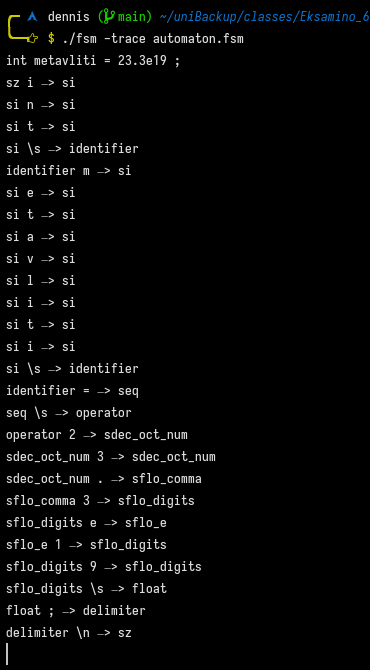
\includegraphics[width=0.5\textwidth]{test_metavliti}
\end{figure}

\begin{figure}[h]
  \caption{Για αποτέλεσμα 6.2}
  \centering
  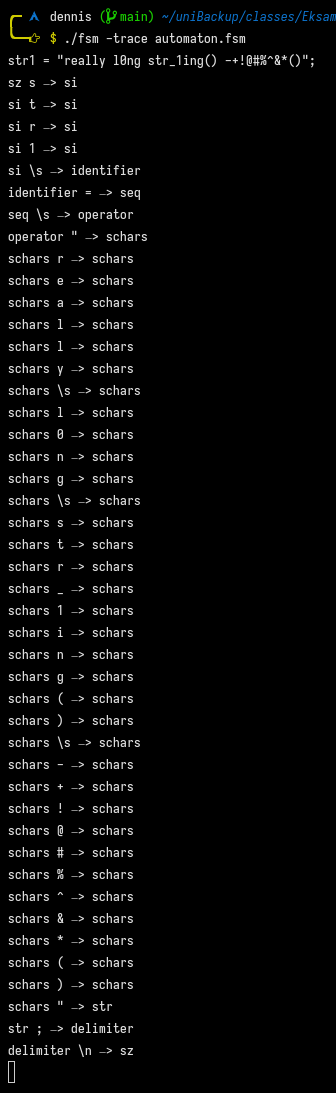
\includegraphics[width=0.45\textwidth]{test_long_string}
\end{figure}

\begin{figure}[h]
  \caption{Για αποτέλεσμα 6.3}
  \centering
  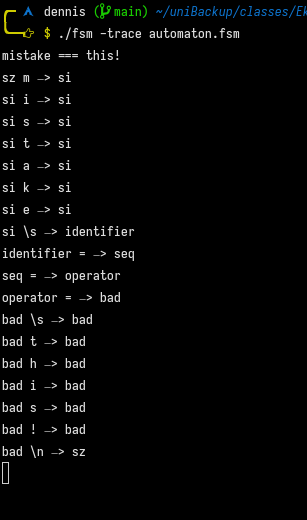
\includegraphics[width=0.5\textwidth]{test_mistake}
\end{figure}

\begin{figure}[hc]
  \caption{Για αποτέλεσμα 6.4}
  \centering
  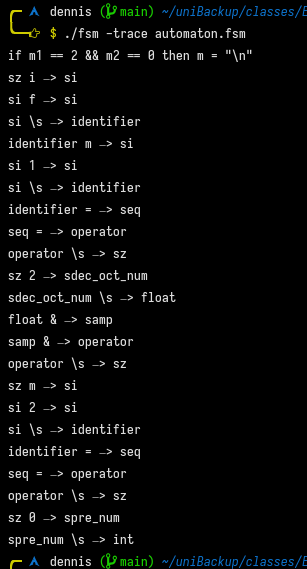
\includegraphics[width=0.5\textwidth]{test_if}
\end{figure}

\end{document}
